% Wie eingangs erwähnt, definieren die Anforderungen, was das System zu
% leisten hat, während die Funktionalitä-ten definieren, wie das System diese gewährleistet.
\chapter{Interface-Design}
\label{chapter-design}
Neben den inhaltlichen Funktionalitäten ist im menschzentrierten Gestaltungsprozess vor allem das
Interface-Design und die Gestaltung der Komponenten von zentraler Bedeutung
\cite{din_en_iso_9421-2102020-03_din_nodate} (DIN EN ISO 9241-210, 2011). Das Design sollte so
entwickelt werden, dass es möglichst optimal die aus \ref{chapter-konzept} entwickelten
Funktionalitäten berücksichtigt. Folglich sollten die in \ref{section:benutzer} erarbeiteten
Nutzenden die Gestaltungslösungen verstehen und bedienen können.

Die Medieninformatik beinhaltet viele Methoden und Vorgehensweisen zur menschzentrierten Gestaltung
\cite{Herczeg2009}. Im Rahmen der Arbeit wurde vor allem Prototyping in verschiedenen Formen
eingesetzt \cite{herczeg_einfuhrung_2009}. Des Weiteren wurden die Zehn Usability Heuristiken nach
\citeA{nielsen_enhancing_1994} bei der Entwicklung stets mit eingearbeitet, um Kriterien der
Gebrauchstauglichkeit zu addressieren \todo{Ausführliche Aufzählung der Heuristiken im Anhang}. In
der Gestaltung wurde nach der \enquote{Mobile First}-Strategie gearbeitet (\anfref{R40}). Diese
besagt die Nutzung der Bildschirmfläche zur schrittweisen Verbesserung von Darstellung und Inhalt
\cite{kim_chapter_2013}. Bei der Anordnung der Komponenten wurde sich an, aus den \ref{subsection:interview}, genannten
Anwendungen, wie Airbnb\footnote{\url{https://www.airbnb.de/}} und
Otto\footnote{\url{https://www.otto.de/}} orientiert. Des Weiteren wurden Tailwind
UI\footnote{\url{https://tailwindui.com/components}} und Headless
UI\footnote{\url{https://headlessui.com/}} als Inspirationsquelle herangezogen, um die Realisierung
des Systems zu erleichtern.

Die erste Iteration des Interface-Designs umfasst Skizzen. Die Skizzen wurden erstellt, um einen
groben Überblick der verschiedenen Ansichten zu erhalten und in
Mockup\footnote{\url{https://getmockup.app/}} umgesetzt. Während des Interface-Designs wurden die
Skizzen mit Figma\footnote{\url{https://www.figma.com/de/}} zu einem High-Fidelity-Prototyp
weiterentwickelt.

Im Rahmen dieses Kapitels werden die zentralen Ansichten und Design Entscheidungen erläutert. Eine
Übersicht aller Entwürfe befindet sich im \todo{Anhang}.

\section{Iteratives Vorgehen}
Für die Tests wurden Usability Spezifikationen aus Szenarien abgeleitet. Die Szenarien beschreiben
Aufgaben, welche als Vorlage dienen können \todo{Anhang, Quelle Scenario Based Design einfügen - auch,
    wenn nicht nach dem Prozess vorgegangen, ist es doch sicherlich eine gute Quelle, die man für die
    Entwicklung von Szenarien zitieren kann}. Um repetitive Evaluationsergebnisse zu verhindern, wurden
die Evaluationsergebnisse kontinuierlich in die weitere Entwicklung eingearbeitet. \ref{table:e}
stellt die Interviewteilnehmenden  mit IDs dar, welche in den folgenden Abschnitten als Verweise
verwendet werden.

\begin{table}[h]
    \centering
    \caption{Teilnehmende der Evaluation}
    \begin{tabular}{lll}
        \arrayrulecolor{maincolor}\hline
        \sffamily\color{maincolor}ID & \sffamily\color{maincolor}Alter &
        \sffamily\color{maincolor}Rolle                                                                           \\
        \arrayrulecolor{maincolor}\hline
        E1                           & 19 - 25 J.                      &
        Medieninformatikerin                                                                                      \\
        E2                           & 19 - 25 J.                      & Robotikerin                              \\
        E3                           & 19 - 25 J.                      & Medieninformatiker, Hilfswissenschaftler \\
        E4                           & 19 - 25 J.                      & Medieninformatiker                       \\
        E5                           & 19 - 25 J.                      &
        Medieninformatikerinnen, Hilfswissenschaftlerin                                                           \\
        E6                           & 25 - 30 J.                      & Wissenschaftlicher Mitarbeiter           \\
        \arrayrulecolor{maincolor}\hline
    \end{tabular}
    \label{table:e}
\end{table}

\section{Designsprache}

Im Folgenden wird auf die Entwicklung der wichtigsten Komponenten und Ansichten in der
Interfacegestaltung eingegangen.

\subsection{Wortlaut}
Ein zentrales Problem des Prototyps war einen konsistenten Wortlaut zu erlangen (H2, H4, H5).
Insbesondere der Begriff \textit{Assets} hat zu Verwirrungen geführt, da nicht klar war, was der
Begriff definiert (E1, E2). Daraufhin wurden Vorschläge geliefert, wie \textit{Material, Hardware,
    Systeme, Geräte}. Im weiteren Verlauf hat sich \textit{Material} als am verständlichsten
herausgestellt (E3-E5). Des Weiteren hat das \textit{Suchen nach Kriterien} für Missverständnisse
und der Parallelen \textit{Suche} ergeben (E1, E2). Daher wurden auch hier verschiedene Begriffe wie
\textit{Auswahlhilfe, Suchhilfe, Kriterien-Suche, Kriterien-Hilfe, Auswahl nach Kriterien, Ausleih-Hilfe}
erarbeitet. Da die Funktion im Rahmen dieser Arbeit nicht Realisierung wird, wurde hier keine
weitere Entscheidung getroffen\todo{Ausblick}.

\subsection{Schrift}
Allgemein wurde die Schriftart nach Kriterien für eine gute Lesbarkeit, wie: Erkennbarkeit,
Unterscheidbarkeit und Offenheit betrachtet \cite{kommunikationsdesign_leserlichinfo}. Außerdem
wurde sich für die spätere Realisierung für die Typografie direkt an Tailwind
UI\footnote{\url{https://tailwindui.com/components}} orientiert und daher Segul UI gewählt.


\subsection{Farbschema}
Die Farben der Anwendung (\ref{fig:farben}) werden nach dem 60-30-10 Prinzip genutzt
\cite{experience_using}. Wobei grau die Hauptfarbe darstellt, weiß die Sekundär Farbe und organe die
Akzentfarbe. Da die Anwendung eine Software am \ac{imis} ist und die Farben des Instituts sich auf
Orange und das Universitäts-Blau beschränken, wurde sich nach einigen Vergleichen für das Orange
entschieden (E4,E5). Der dunkle Ton stellt die Textfarbe der Anwendung dar.
\begin{figure}[h]
    \centering
    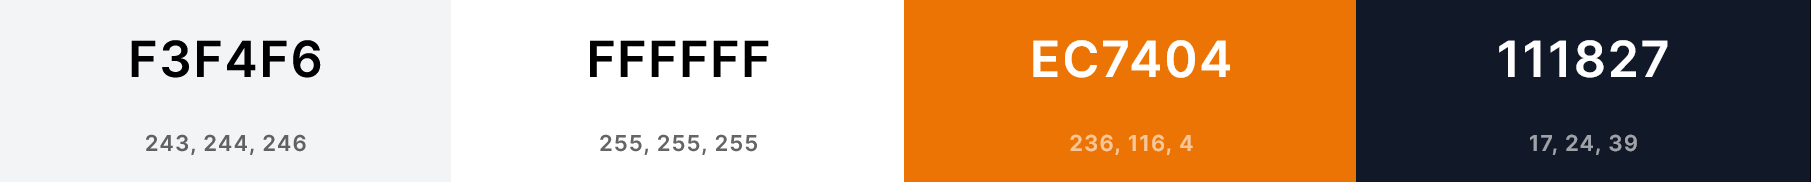
\includegraphics[scale=0.23]{Bilder/farben.png}
    \caption[Farbpalette]{Farbpalette}
    \label{fig:farben}
\end{figure}

\subsection{Dashboard}
Positiv wurde stets angemerkt, dass die Anwendung im allgemeinen sauber und nicht überladen wirkt (H8)
(E1-6). Aufgrund des zu Beginn geringen Inhalts auf der Startseite ist eine ansprechende und
fokussierte Anordnungen der Komponenten wichtig (H8). \ref{fig:home} zeigt die Entwicklung des
Dashboards. Ein wichtiger Punkt war die im linken Bild fehlende Orientierung (E1-4). Außerdem
wirkte die Ansicht durch die vielen einzelnen Elemente schnell überladen (H8) (E1-2). Daher wurde
sich für eine simple Tab-Leiste entschieden. Folglich ist die Seite auch bei mehr als drei
Reservierungen übersichtlich (E4). Sobald ein Asset ausgeliehen wurde, sollten die entsprechenden
Informationen (Status, Zeitraum, Ort) übersichtlich und schnell eingesehen werden können (H1)
(F-A-1). Dies ermöglicht die Kartenansicht, wobei eine Möglichkeit zum Löschen und das Bearbeiten
des Zeitraums erwünscht war und in der Realisierung integriert wurde (E6).

Die Verwaltungsansicht, in welcher die Möglichkeit zum Aktualisierendes Status besteht, entspricht zum
Großteil dem Dashboard (H6) (F-V-1, F-V-2).

\begin{figure}[h]
    \centering
    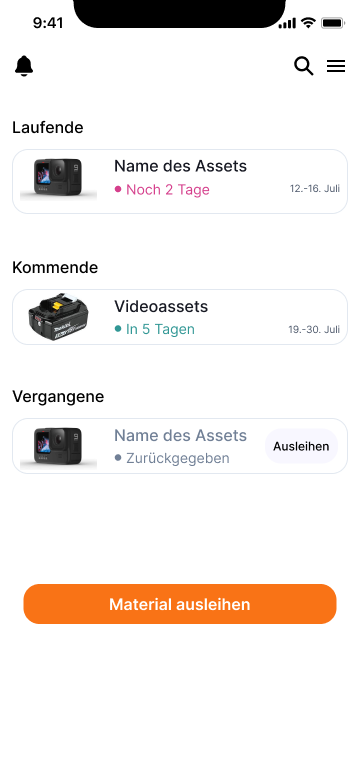
\includegraphics[scale=0.4]{Bilder/Prototyp/Start.png}\hspace{2em}
    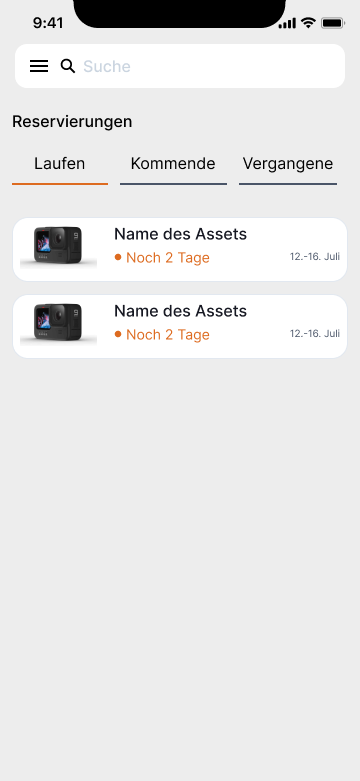
\includegraphics[scale=0.4]{Bilder/Prototyp/Neu/V2.png}
    \caption[-]{Navigationsmöglichkeiten}
    \label{fig:home}
\end{figure}

\subsection{Navigation und Suchleiste}
In der Interface-Gestaltung gibt es verschiedene Möglichkeiten Navigation bereitzustellen. Für die
Anwendung wurde für den Mobilen Kontext eine Navigationsleiste am unteren Bildschirmrand und ein
Burgermenü in Erwägung gezogen. Für die Desktop-Navigation wurde zwischen einer festen
Navigationsleiste links und einer Leiste oben abgewägt (\ref{fig:nav}). An Ende wurde sich für eine
Navigationsleiste auf der linken Seite entscheiden. Orientiert wurde sich hierbei an bekannten
Anwendungen mit ähnlichen Funktionen und dem Material Design \cite{google_material_2022}. Die
Umgangsweise mit diesen Gestaltungslösungen ist bereits bekannt und somit übertragbar (H4, H6).
Daran anknüpfend wurde sich für eine integrierte Suchleiste entschieden, sodass Nutzende jederzeit
die Möglichkeit haben, nach Assets zu suchen \cite{google_material_2022} (E4).


\begin{figure}[h]
    \centering
    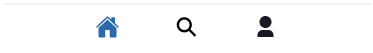
\includegraphics[scale=0.3]{Bilder/Prototyp/Property 1=Variant2.png} \hspace{2em}
    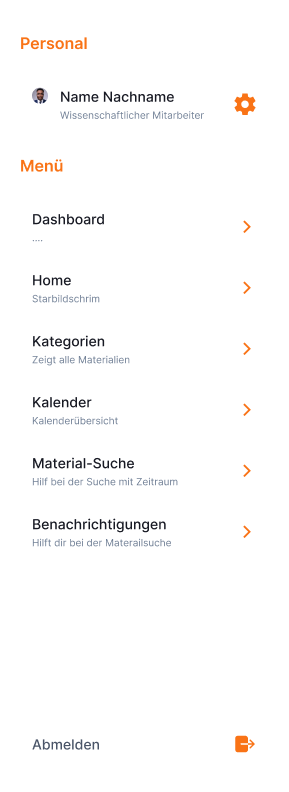
\includegraphics[scale=0.4]{Bilder/Prototyp/Menu.png} \hspace{2em}
    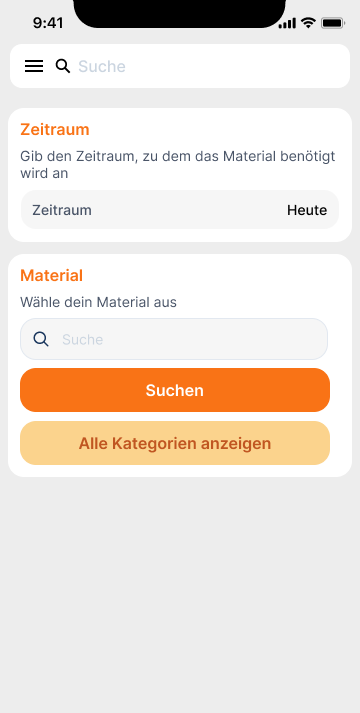
\includegraphics[scale=0.4]{Bilder/Prototyp/Neu/Suche V2.png}
    \caption[-]{Navigationsmöglichkeiten}
    \label{fig:nav}
\end{figure}

\subsection{Kategorien und Suche}
Die Übersicht der Kategorien sind auch hier wieder an bekannten Anwendungen mit ähnlichen Funktionen
angelehnt (H4, H8). Dies führt unter anderem auch dazu, dass Fehler vermieden werden können (H9).

Die Suche ist durch die Anwendung Airbnb\footnote{\url{https://www.airbnb.de/}} entstanden, da viele
Nutzende beim Reservieren die Anwendung assoziieren (H2, H4). Die Suche sollte durch das direkte
Einstellen eines Ausleihzeitraums Fehler vorbeugen und Verfügbarkeit anzeigen (H5) (F-VA-6).
\ref{fig:p1} zeigt die erste Version des High-Fidelity-Prototypen, bei welcher zum einen ein
Suchbutton fehlte, zudem wurden die Vorschläge der angezeigten Kategorien weniger genutzt wurden und
direkt auf die Suche oder \textit{alle Kategorien Anzeigen} geklickt wurde, daher wurden diese
Elemente entsprechenden angepasst (E1, E2, E4).

\begin{figure}[h]
    \centering
    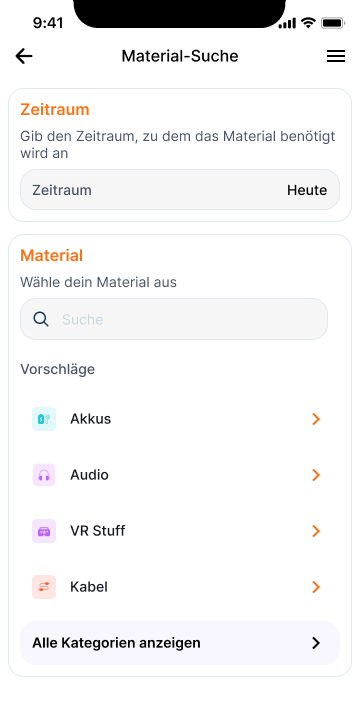
\includegraphics[scale=0.3]{Bilder/Prototyp/Suche.png}\hspace{2em}
    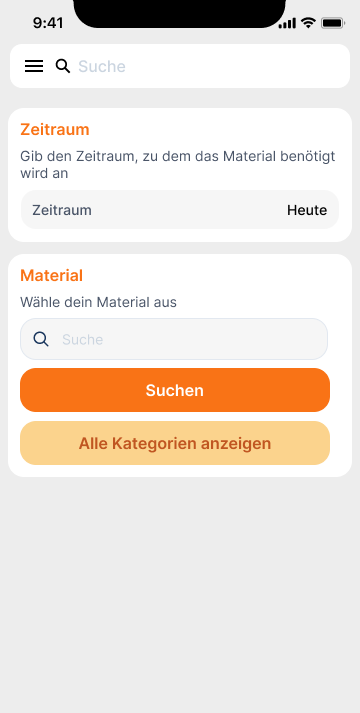
\includegraphics[scale=0.3]{Bilder/Prototyp/Neu/Suche V2.png}\hspace{2em}
    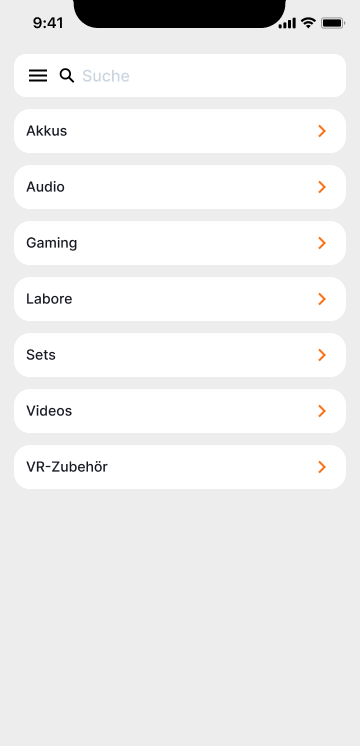
\includegraphics[scale=0.3]{Bilder/Prototyp/Neu/Kategorein 1.png}
    \label{fig:p1}
    \caption[Mockup: Kategorien, Assets, Assetdetails]{Kategorien (l), Assets (m), Assetdetails (r)}
\end{figure}

Für eine Unteransicht wurde sich für eine Kartenansicht entscheiden (ref{fig:p4}). Diese ergab sich aus dem
bereits bekannten Prinzipen von Online-Einkäufen. Dem Nutzenden wird mithilfe eines Bildes direkt
gezeigt, um was für ein Asset es sich handelt. Außerdem wird auch hier die Assetverfügbarkeit mit
eingebunden (H4, H8) (F-VA-3).

\begin{figure}[h]
    \centering
    \includegraphics[scale=0.3]{Bilder/Prototyp/Übersicht.png}\hspace{2em}
    \includegraphics[scale=0.3]{Bilder/Prototyp/Übersicht1.png}
    \label{fig:p4}
    \caption[Mockup: Kategorien, Assets, Assetdetails]{Kategorien (l), Assetdetails (r)}
\end{figure}


\subsection{Kalender}
Die Kalenderkomponente wurde lediglich als Skizze veranschaulicht (\ref{fig:kalender}). In den High-Fidelity-Prototyp
wurde sich bereits an der Komponenten \textit{V-Calendar}\footnote{\url{https://vcalendar.io/layouts.html}}
orientiert, welche die wichtigsten Funktionen mitbrachte und so die Realisierung erleichtert.

Bei dem Kalender war es unter anderem wichtig, dass Wochenenden ausgeblendet werden können, da zu
diesen Zeitpunkten keine Ausleihe möglich ist (H1) (F-VA-3). Außerdem sollten vergangene Tage nicht
auswählbar sein. Weitere Punkte wurden auch hier wieder von der Anwendung Airbnb berachtet (H4, H7,
H8) (E2-4).

Für Verleihende ist eine generelle Übersicht, über einzelne Tage wichtig, um Abholungen und
Rückgaben von Assets besser planen zu können (F-V-4).

\begin{figure}[h]
    \centering
    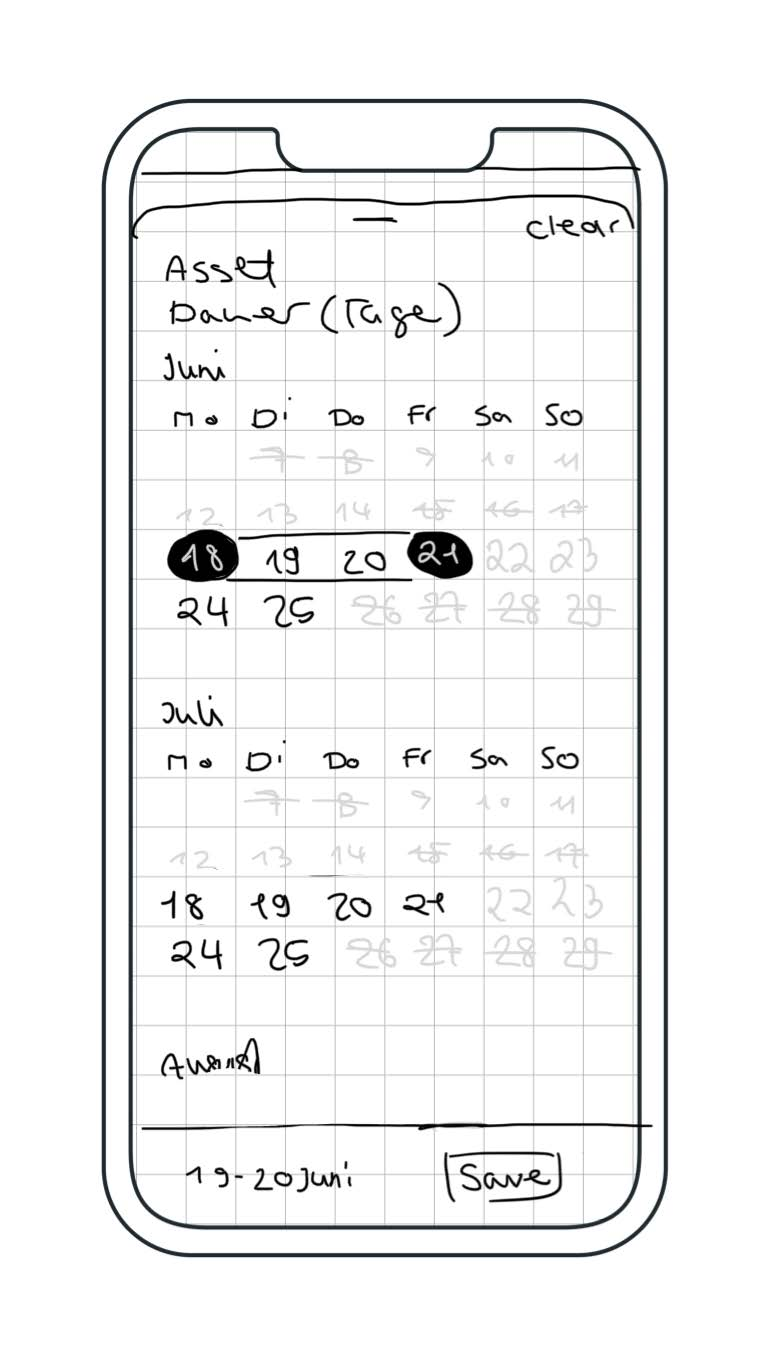
\includegraphics[scale=0.4]{Bilder/Mockups/Kalender.jpg}\hspace{2em}
    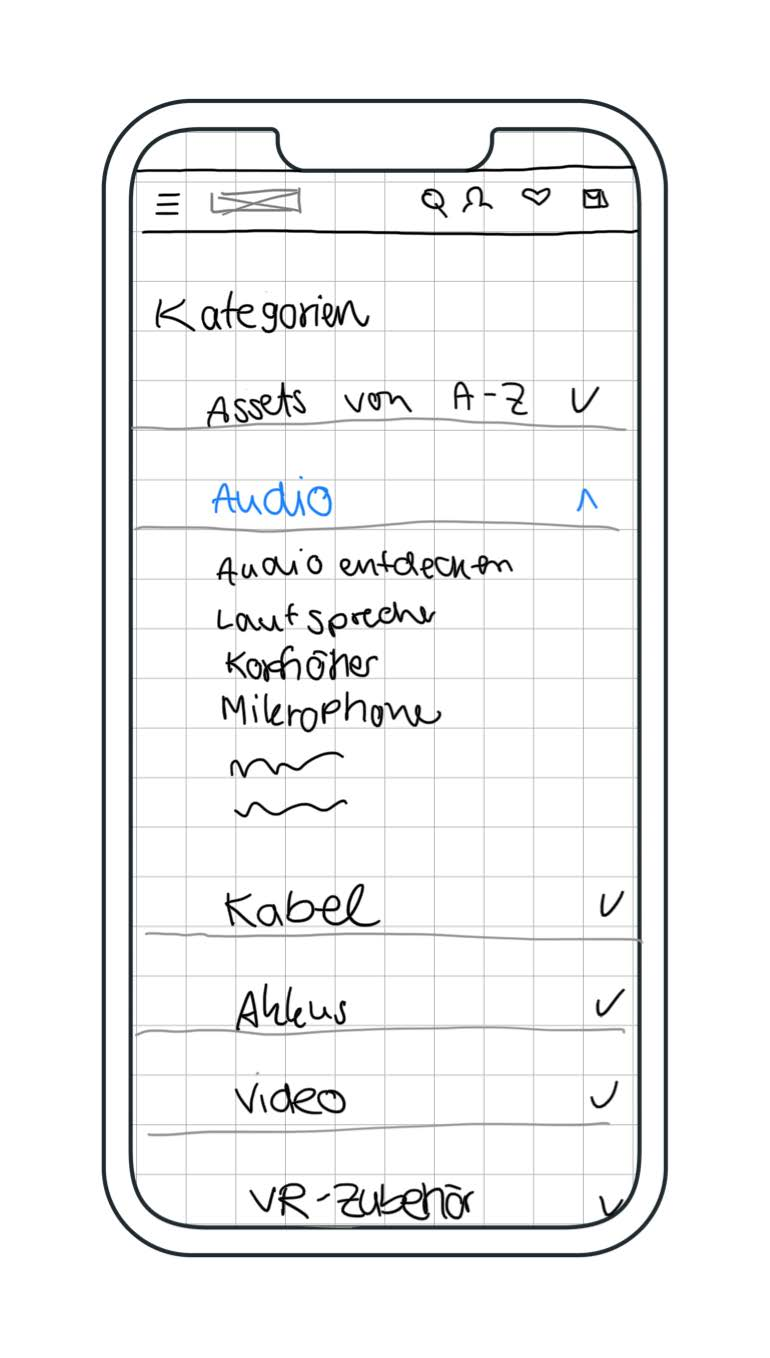
\includegraphics[scale=0.4]{Bilder/Mockups/Kategorien.jpg}
    \label{fig:kalender}
    \caption[Kalenderkomponente]{Kalender (l), Navigation (r)}
\end{figure}

\subsection{Asset-Detailansicht und Reservierungen}
Die Ansicht der einzelnen Assets sollte insbesondere Assetverfügbarkeit, Funktionalitäten sowie
Verleihende enthalten (F-VA-3, F-VA-4, F-VA-8). \ref{fig:p3} zeigt die genannten Informationen. Es
ergab sich, dass eine Assetbeschreibung des Artikels zunächst nicht von Bedeutung sei (E6). Den
Ausleihzeitraum separat zur Abholung und Rückgabe anzeigen zu lassen führte im Verlauf häufig zu
Verwirrung, daher wurden die zeitlichen Daten auf die Abholung und Rückgabe beschränkt (H5) (E5, E6).

\begin{figure}[h]
    \centering
    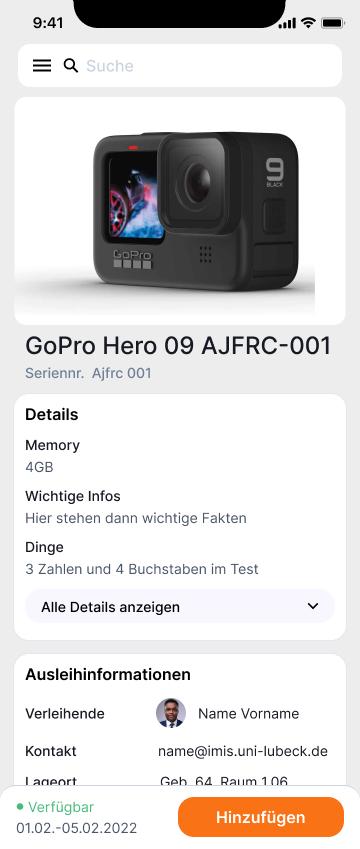
\includegraphics[scale=0.3]{Bilder/Prototyp/Neu/Datailansicht-1.png}\hspace{2em}
    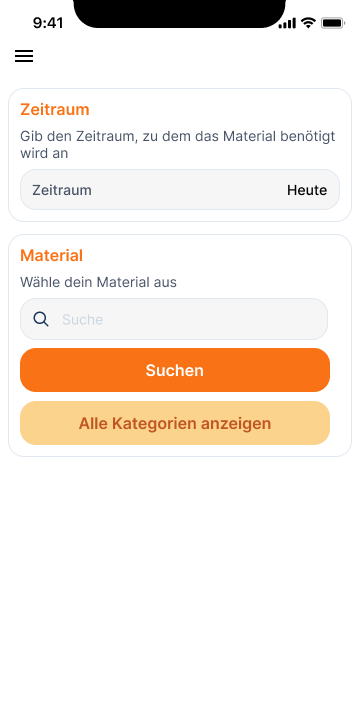
\includegraphics[scale=0.3]{Bilder/Prototyp/Neu/Suche.png}\hspace{2em}
    \includegraphics[scale=0.3]{Bilder/Prototyp/Reservierung abschließen 3.png}
    \label{fig:p3}
    \caption[Mockup: Kategorien, Assets, Assetdetails]{Kategorien (l), Assets (m), Assetdetails (r)}
\end{figure}